\documentclass[a4paper]{article}
\usepackage[utf8]{inputenc}
\usepackage[russian,english]{babel}
\usepackage[T2A]{fontenc}
\usepackage[left=10mm, top=20mm, right=18mm, bottom=15mm, footskip=10mm]{geometry}
\usepackage{indentfirst}
\usepackage{amsmath,amssymb}
\usepackage{mathastext} 
\usepackage[italicdiff]{physics}
\usepackage{graphicx}
\usepackage{caption}
\usepackage{float}
\usepackage{caption}
\renewcommand{\thefootnote}{\fnsymbol{footnote}}
\usepackage{tablefootnote}
\usepackage{footmisc}
\usepackage{textcomp}
\usepackage{multicol}
\usepackage{multirow}
\usepackage[parfill]{parskip}
\usepackage{makecell}
\usepackage{array}  
\usepackage{siunitx}
\usepackage{booktabs}
\sisetup{
    exponent-product = \cdot,
    per-mode = symbol,
    separate-uncertainty = true,
    uncertainty-separator = \,
}
\renewcommand\cellalign{cc} 
\renewcommand\cellgape{\Gape[2pt]} 
\usepackage[utf8]{inputenc}\newcommand{\approxtext}[1]{\ensuremath{\stackrel{\text{#1}}{\approx}}}
\usepackage[colorlinks=true, urlcolor=blue, linkcolor=blue, citecolor=blue]{hyperref}
\graphicspath{{images/}}
\DeclareGraphicsExtensions{.pdf,.png,.jpg}
\usepackage{wrapfig}
\captionsetup{labelformat=empty}
\usepackage{caption}
\captionsetup[figure]{name=Рисунок}
\captionsetup[table]{name=Таблица}
%\usepackage{newtxtext,newtxmath} 
\title{\textbf{Отчет о выполнении лабораторной работы 3.2.6}}
\date{}
\author{Котляров Михаил, Б01-402}

\begin{document}

\maketitle
	
\section{Введение}

\subsubsection*{Цель работы}
Изучение работы высокочувствительного зеркального гальванометра магнитоэлектрической системы в режимах измерения постоянного тока и электрического заряда.

\subsubsection*{Оборудование}
\begin{itemize}
    \item Зеркальный гальванометр с осветителем и шкалой
    \item Источник постоянного напряжения
    \item Делитель напряжения
    \item Магазин сопротивлений
    \item Эталонный конденсатор
    \item Вольтметр
    \item Переключатель
    \item Ключи
    \item Линейка
\end{itemize}

\section{Экспериментальная установка}

\subsection{Определение динамической постоянной}

\begin{figure}[h]
    \centering
    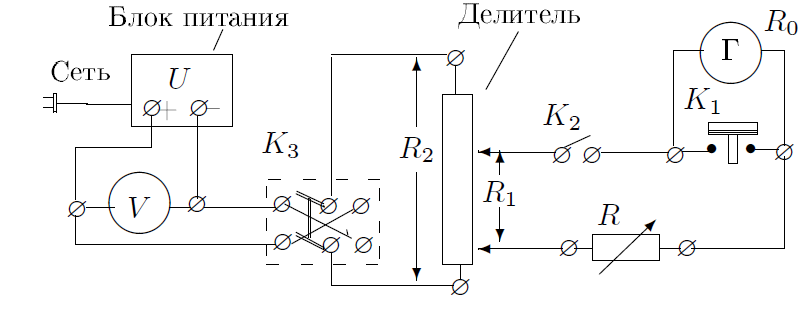
\includegraphics[width=10cm]{Pictures/ustanovka_stat.PNG}
    \caption{Рис. 1. Схема установки для работы гальванометра в стационарном режиме}
    \label{fig:scheme1}
\end{figure}

Схема для исследования гальванометра в стационарном режиме представлена на рис. \ref{fig:scheme1}. Постоянное напряжение $U = 1,5$ В снимается с блока питания и измеряется вольтметром $V$. Ключ $K_3$ позволяет менять направление тока через гальванометр $\Gamma$, делитель напряжения --- менять величину тока в широких пределах. Ключ $K_2$ служит для включения гальванометра, кнопка $K_1$ --- для его успокоения. Магазин сопротивлений $R$ позволяет менять режим работы гальванометра от колебательного до апериодического.

При $R_1 \ll R, R_0, R_2$ сила тока, протекающего через гальванометр, может быть вычислена по формуле:
\begin{equation}
    I = U_0 \frac{R_1}{R_2} \frac{1}{R + R_0}.
    \label{eq:current}
\end{equation}

Угол отклонения рамки от положения равновесия измеряется с помощью осветителя, зеркальца, укреплённого на рамке, и шкалы. Координата $x$ светового пятна на шкале связана с углом $\varphi$ отклонения рамки формулой:
\[
x = a \arctg 2\varphi,
\]
где $a$ --- расстояние от шкалы до зеркальца. При малых углах $\varphi = x/2a$. Динамическую постоянную вычисляют по формуле:
\begin{equation}
    C_I = \frac{I}{\varphi} = \frac{2aI}{x}.
    \label{eq:dyn_const}
\end{equation}

\subsection{Определение критического сопротивления гальванометра}

Измерение критического сопротивления гальванометра выполняется с помощью той же схемы (рис. \ref{fig:scheme1}). При больших $R$ свободное движение рамки имеет колебательный характер. С уменьшением $R$ затухание увеличивается, и колебательный режим переходит в апериодический.

В качестве характеристики процесса затухания колебаний рамки гальванометра используют логарифмический декремент затухания:
\begin{equation}
    \Theta = \ln\frac{x_n}{x_{n+1}} = \gamma T = \frac{2\pi \gamma}{\sqrt{\omega_0^2 - \gamma^2}} = \frac{2\pi (R_{\text{кр}} + R_0)}{\sqrt{(R_0 + R)^2 - (R_{\text{кр}} + R_0)^2}},
    \label{eq:decrement}
\end{equation}
где $x_n$ и $x_{n+1}$ --- два последовательных отклонения зайчика в одну сторону.

Критическое сопротивление рассчитывают по графику в координатах $X = (R_0 + R)^2$, $Y = 1/\Theta^2$:
\begin{equation}
    R_{\text{кр}} = \frac{1}{2\pi}\sqrt{\frac{\Delta X}{\Delta Y}} - R_0.
    \label{eq:crit_res}
\end{equation}

\subsection{Определение баллистической постоянной и критического сопротивления гальванометра, работающего в баллистическом режиме}

\begin{figure}[h]
    \centering
    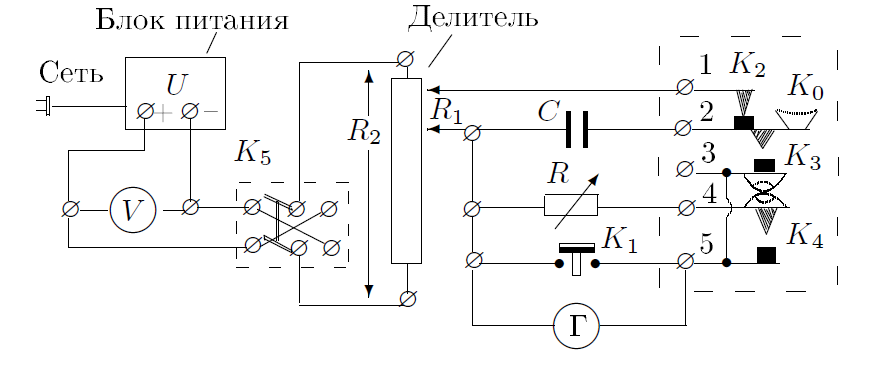
\includegraphics[width=10cm]{Pictures/ustanovka_ball.PNG}
    \caption{Рис. 2. Схема установки для определения баллистической постоянной}
    \label{fig:scheme2}
\end{figure}

Для изучения работы гальванометра в режиме измерения заряда используется схема, представленная на рис. \ref{fig:scheme2}. 

При нормальном положении кнопки $K_0$ конденсатор $C$ заряжается до напряжения:
\[
U_c = \frac{R_1}{R_2}U_0.
\]
Заряд конденсатора равен:
\[
q = \frac{R_1}{R_2}U_0 C.
\]

При нажатии на ключ $K_0$ конденсатор отключается от источника постоянного напряжения и подключается к гальванометру. К моменту замыкания ключа $K_4$ весь заряд успевает пройти через гальванометр, и рамка получает начальную скорость.

Баллистическая постоянная гальванометра определяется при критическом сопротивлении:
\begin{equation}
    C_Q^{кр} = \frac{q}{\varphi_{max}^{кр}} = 2a\frac{R_1}{R_2} \frac{U_0 C}{l_{max}^{кр}},
    \label{eq:ball_const}
\end{equation}
где $l_{max}^{кр}$ --- величина первого отброса в критическом режиме, выраженная в делениях шкалы.

\section{Теоретические сведения}

Баллистический гальванометр --- электроизмерительный прибор магнитоэлектрической системы, отличающийся высокой чувствительностью к току и сравнительно большим периодом колебаний подвижной системы (рамки). Главной частью прибора является подвешенная на вертикальной нити рамка, помещённая в поле постоянного магнита.

Движение рамки описывается уравнением:
\[
\ddot{\varphi} + 2\gamma \dot{\varphi} + \omega_0^2 \varphi = KI,
\]
где $\varphi$ --- угол поворота рамки, $\gamma$ --- коэффициент затухания, $\omega_0$ --- собственная частота колебаний, $K$ --- постоянная, зависящая от параметров гальванометра.

В работе исследуются два основных режима:
\begin{enumerate}
    \item \textbf{Стационарный режим} --- измерение постоянного тока. Угол отклонения рамки пропорционален току:
    \[
    \varphi = \frac{BSN}{D} I = S_I I = \frac{I}{C_I},
    \]
    где $S_I$ --- чувствительность к току, $C_I$ --- динамическая постоянная гальванометра.
    
    \item \textbf{Баллистический режим} --- измерение электрического заряда. При пропускании короткого импульса тока максимальное отклонение рамки пропорционально прошедшему заряду:
    \[
    \varphi_{\text{max}} = \frac{K}{\omega_0} q = \frac{q}{C_q},
    \]
    где $C_q$ --- баллистическая постоянная гальванометра.
\end{enumerate}

Критическое сопротивление $R_{\text{кр}}$ определяет переход между колебательным и апериодическим режимами работы гальванометра. В критическом режиме обеспечивается оптимальное сочетание чувствительности и времени успокоения прибора.



\section{Выполнение}

\subsection*{Подготовка приборов к работе}
\begin{enumerate}
\item Настроим осветитель гальванометра, добившись появления чёткой вертикальной риски на шкале и совместив её с нулевым делением. Установим делитель на выходное напряжение $\frac{R_1}{R_2} = \frac{1}{1000}$ и сопротивление магазина $R \approx 50$ кОм. Соберём электрическую цепь согласно схеме, включим блок питания и осветитель. Подберём сопротивление магазина, при котором зайчик отклоняется почти на всю шкалу.

\subsection*{Определение динамической постоянной}

\item Измерим зависимость отклонения зайчика $x$ от сопротивления магазина $R$ при постоянном положении делителя. Получили ряд значений сопротивлений и соответствующих им отклонений зайчика. 

Рассчитаем ток через гальванометр для каждого измерения по формуле:
\[
I = U_0 \frac{R_1}{R_2} \frac{1}{R + R_0}
\]
где $U_0 = 1,32 \pm 0,02$ В, $\frac{R_1}{R_2} = \frac{1}{1000}$, $R_0 = 500$ Ом. Погрешность $\sigma_x = 0,1$ см.
\clearpage
\begin{table}[h!]
    \centering
    \begin{tabular}{|c|c|c|}
        \hline
        № & $x$, см & $I$, нА \\ \hline
        1 & 25,0 & 64,39 \\ \hline
        2 & 21,9 & 56,17 \\ \hline
        3 & 19,6 & 49,81 \\ \hline
        4 & 17,7 & 44,75 \\ \hline
        5 & 16,2 & 40,62 \\ \hline
        6 & 14,9 & 37,18 \\ \hline
        7 & 13,7 & 34,29 \\ \hline
        8 & 12,6 & 31,81 \\ \hline
        9 & 11,7 & 29,66 \\ \hline
        10 & 10,9 & 27,79 \\ \hline
        11 & 10,1 & 26,14 \\ \hline
    \end{tabular}
    \caption{Таблица 1. Зависимость отклонения зайчика от силы тока}
    \label{tab:current_deflection}
\end{table}

\item Построим график зависимости $I(x)$ и определим, что зависимость является линейной в рабочем диапазоне отклонений. 
 \begin{figure}[h]
      \center{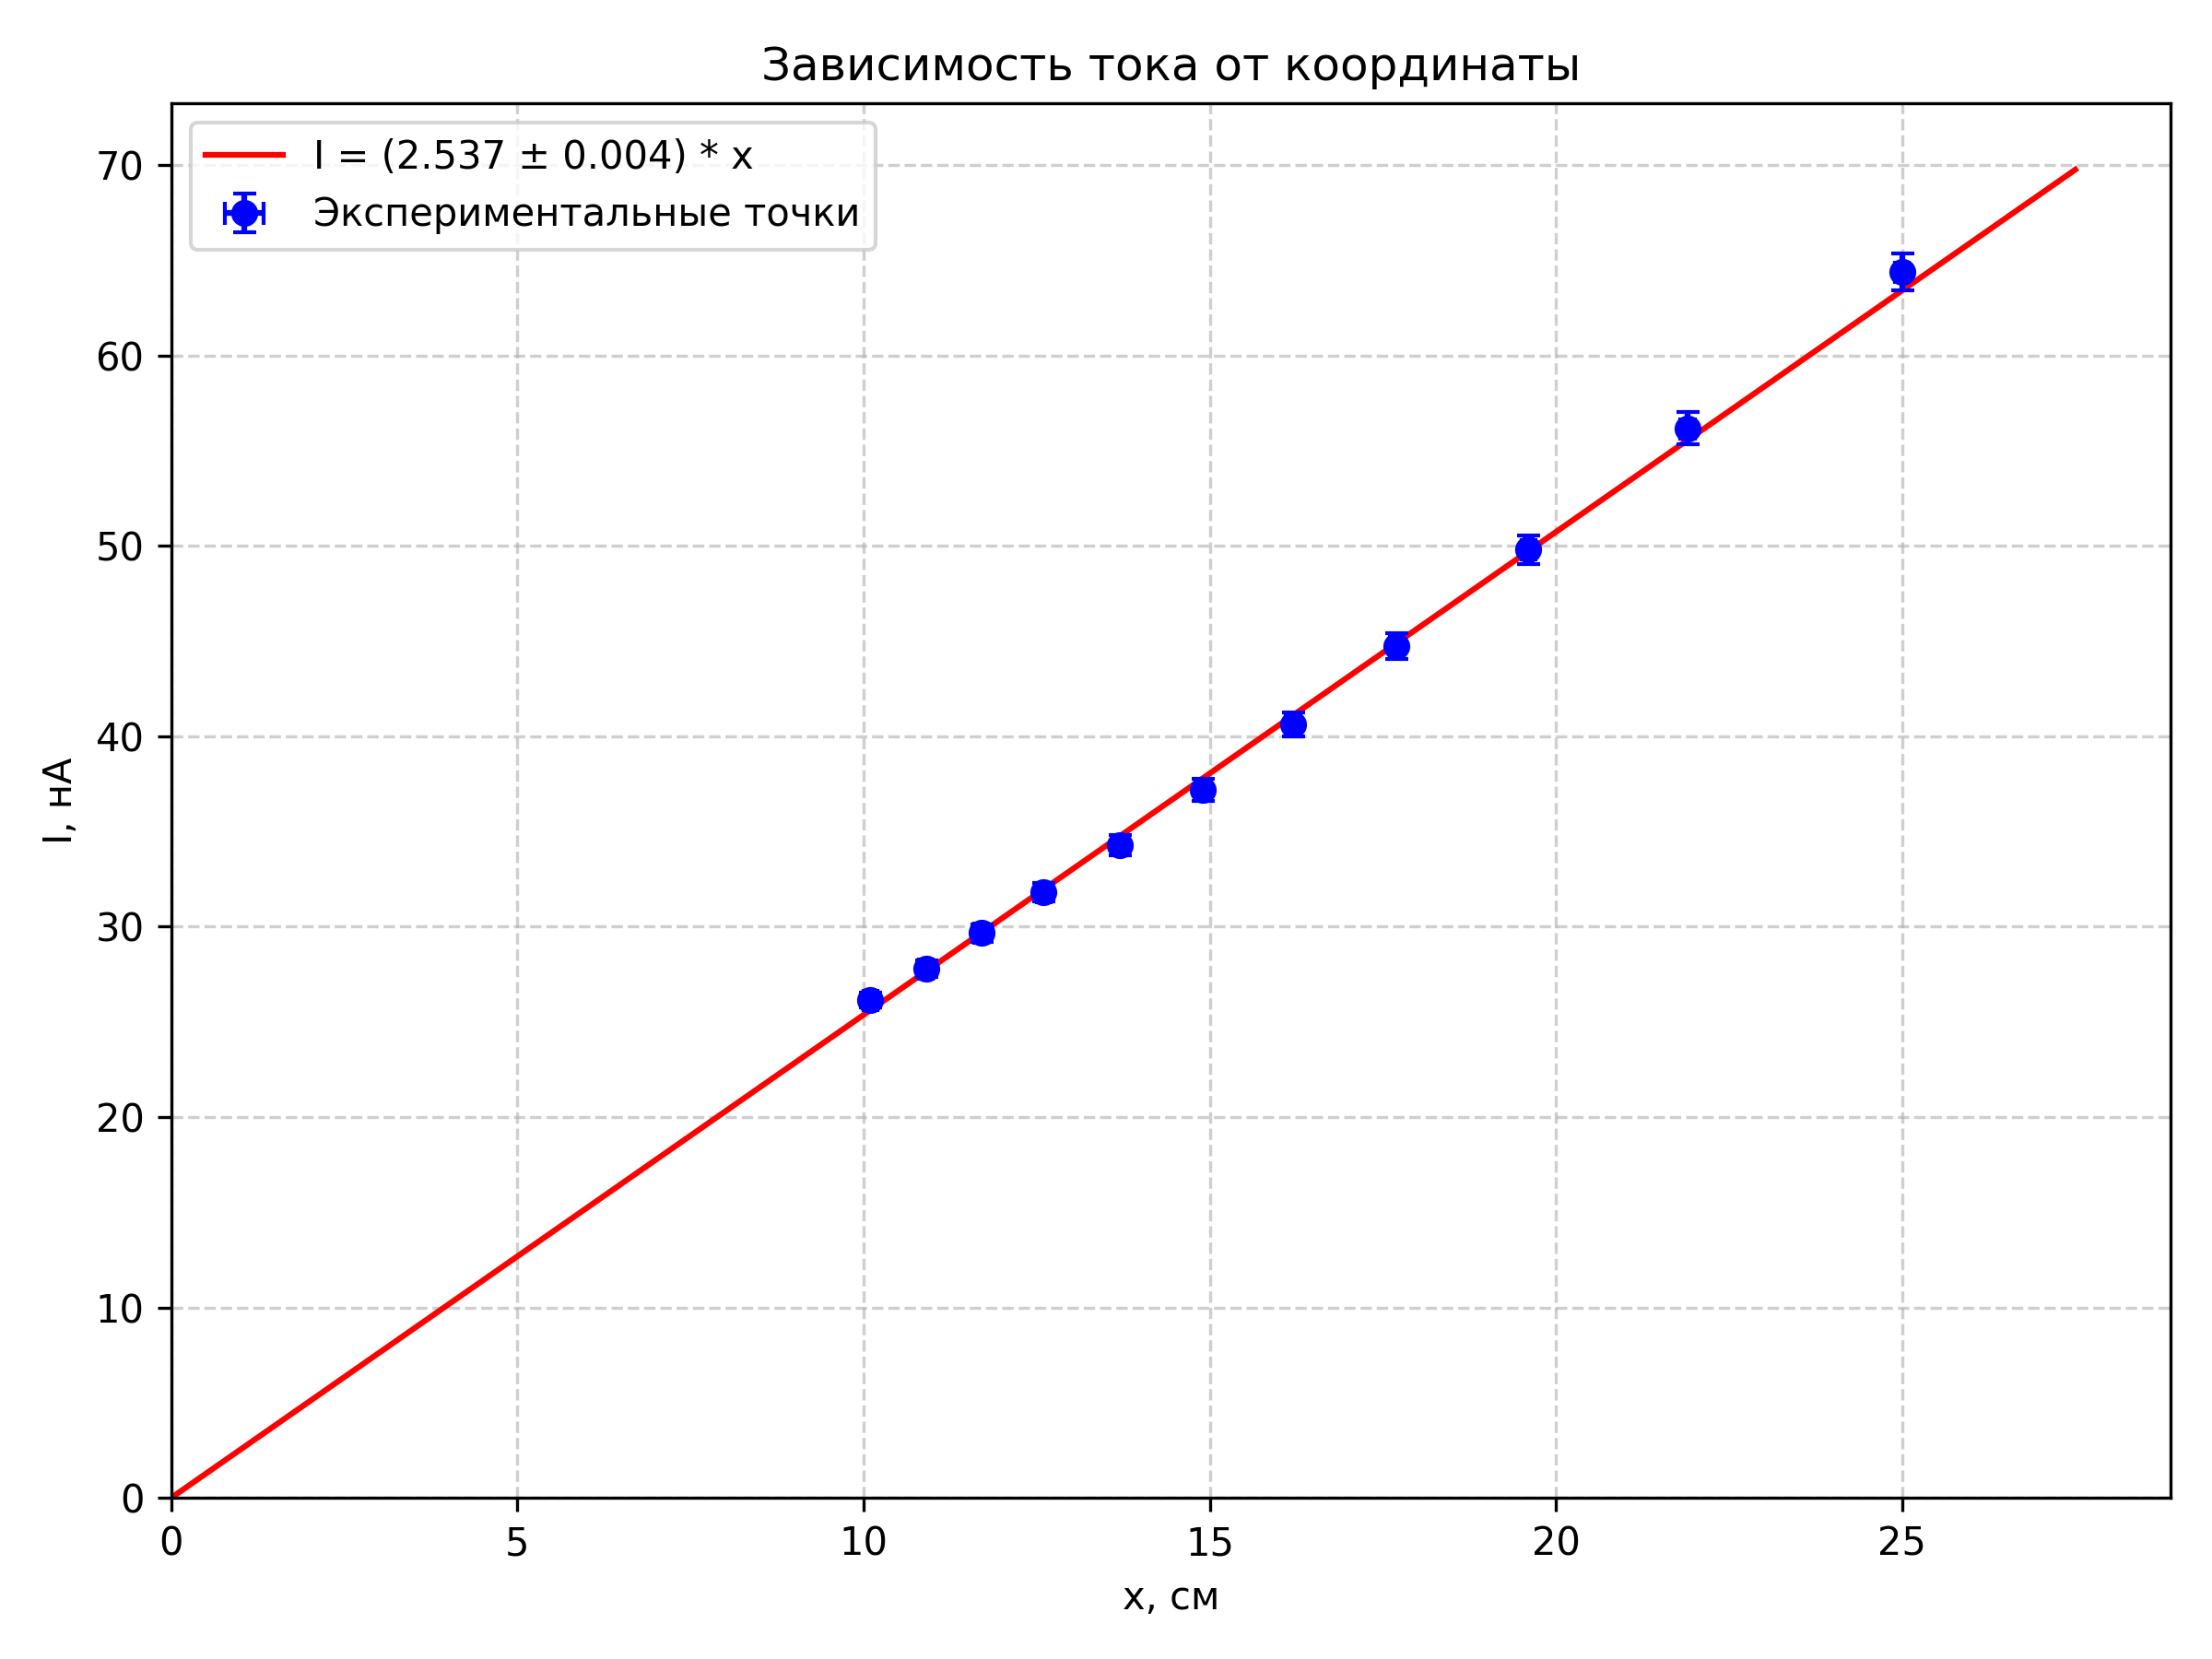
\includegraphics[width=0.7\textwidth]{Graphics/I_vs_x.png}}
      \caption{График 1. Зависимость силы тока от отклонения зайчика}
\end{figure}

Наклон прямой $k = 0,2537 \pm 0,0004 \ \frac{\text{нА}}{\text{мм}}$ ($\varepsilon_k = 0,16 \%$).
По угловому коэффициенту прямой рассчитаем динамическую постоянную:
\[
C_I = \frac{2aI}{x} = 0,120 \pm 0,001 \ \frac{\text{нА}}{\frac{\text{мм}}{\text{м}}},
\]
где $a = 1,06 \pm 0,01$ м -- расстояние от шкалы до гальванометра.
\subsection{Определение критического сопротивления}

\item Исследуем свободные колебания рамки при разомкнутой внешней цепи ($R = \infty$). Измерим последовательные отклонения зайчика в одну сторону: 
\clearpage
\begin{table}[h!]
    \centering
    \begin{tabular}{|c|c|c|}
        \hline
        $n$ & $x$, см & $\Theta$ \\ \hline
        1 & 19,7 & --- \\ \hline
        2 & 16,7 & 0,165 \\ \hline
        3 & 12,5 & 0,290 \\ \hline
        4 & 9,8 & 0,243 \\ \hline
        5 & 8,9 & 0,096 \\ \hline
        6 & 6,3 & 0,346 \\ \hline
        7 & 5,2 & 0,192 \\ \hline
        8 & 4,2 & 0,214 \\ \hline
        9 & 3,4 & 0,211 \\ \hline
        10 & 2,7 & 0,231 \\ \hline
        11 & 2,2 & 0,205 \\ \hline
    \end{tabular}
    \caption{Таблица 2. Логарифмический декремент затухания для различных отклонений}
    \label{tab:decrement_values}
\end{table}

Рассчитаем среднее: $\Theta_0 = 0,219 \pm 0,0231$ ($\varepsilon_{\Theta_0} = 10,56 \%$). Погрешность скадывалась из систематической (с учетом $\sigma_x = 0,2$ см) и случайной.

\item Измерим период свободных колебаний рамки: $T_{11} = 49,23$ с, $T_1 = \frac{T_{11}}{11} = 4,48 \pm 0,05$ с, $\sigma_{T_1} = \frac{\sigma_{T_{11}}}{11} = \frac{0,5}{11} \approx 0,05$.

\item Подберём наибольшее сопротивление магазина $R$, при котором при размыкании ключа зайчик не переходит за нулевое значение. Получили $R_{\text{кр}}^{\text{подб}} \approx 7,5 \pm 0,5$ кОм.

\item Проведём серию измерений логарифмического декремента затухания $\Theta$ для различных значений сопротивления $R$ в диапазоне от $3R_{кр}^{подб}$ до $10R_{кр}^{подб}$.

\begin{table}[h!]
    \centering
    \begin{tabular}{|c|c|c|c|c|c|c|}
        \hline
        № & $X_1$, см & $X_2$, см & $R$, кОм & $R_1/R_2$ & $1/\Theta^2$ & $(R+R_0)^2$, кОм$^2$ \\ \hline
        1 & 6,8 & 0,7 & 23 & 0,001 & $0,193 \pm 0,024$ & 552,25 \\ \hline
        2 & 6,7 & 0,9 & 27 & 0,001 & $0,248 \pm 0,028$ & 756,25 \\ \hline
        3 & 6,8 & 1,2 & 31 & 0,001 & $0,332 \pm 0,032$& 992,25 \\ \hline
        4 & 10,3 & 2,5 & 38 & 0,002 & $0,499 \pm 0,029$& 1482,25 \\ \hline
        5 & 9,5 & 2,9 & 46 & 0,002 & $0,710 \pm 0,043$ & 2162,25 \\ \hline
        6 & 13,0 & 4,5 & 53 & 0,003 & $0,889 \pm 0,039$& 2862,25 \\ \hline
        7 & 13,7 & 6,2 & 75 & 0,005 & $1,591 \pm 0,071$& 5700,25 \\ \hline
    \end{tabular}
    \caption{Таблица 3. Зависимость параметров колебаний от сопротивления цепи}
    \label{tab:resistance_dependence}
\end{table}

По МНК построим график $\frac{1}{\Theta^2} = f((R+R_0)^2)$.
\clearpage
 \begin{figure}[h]
      \center{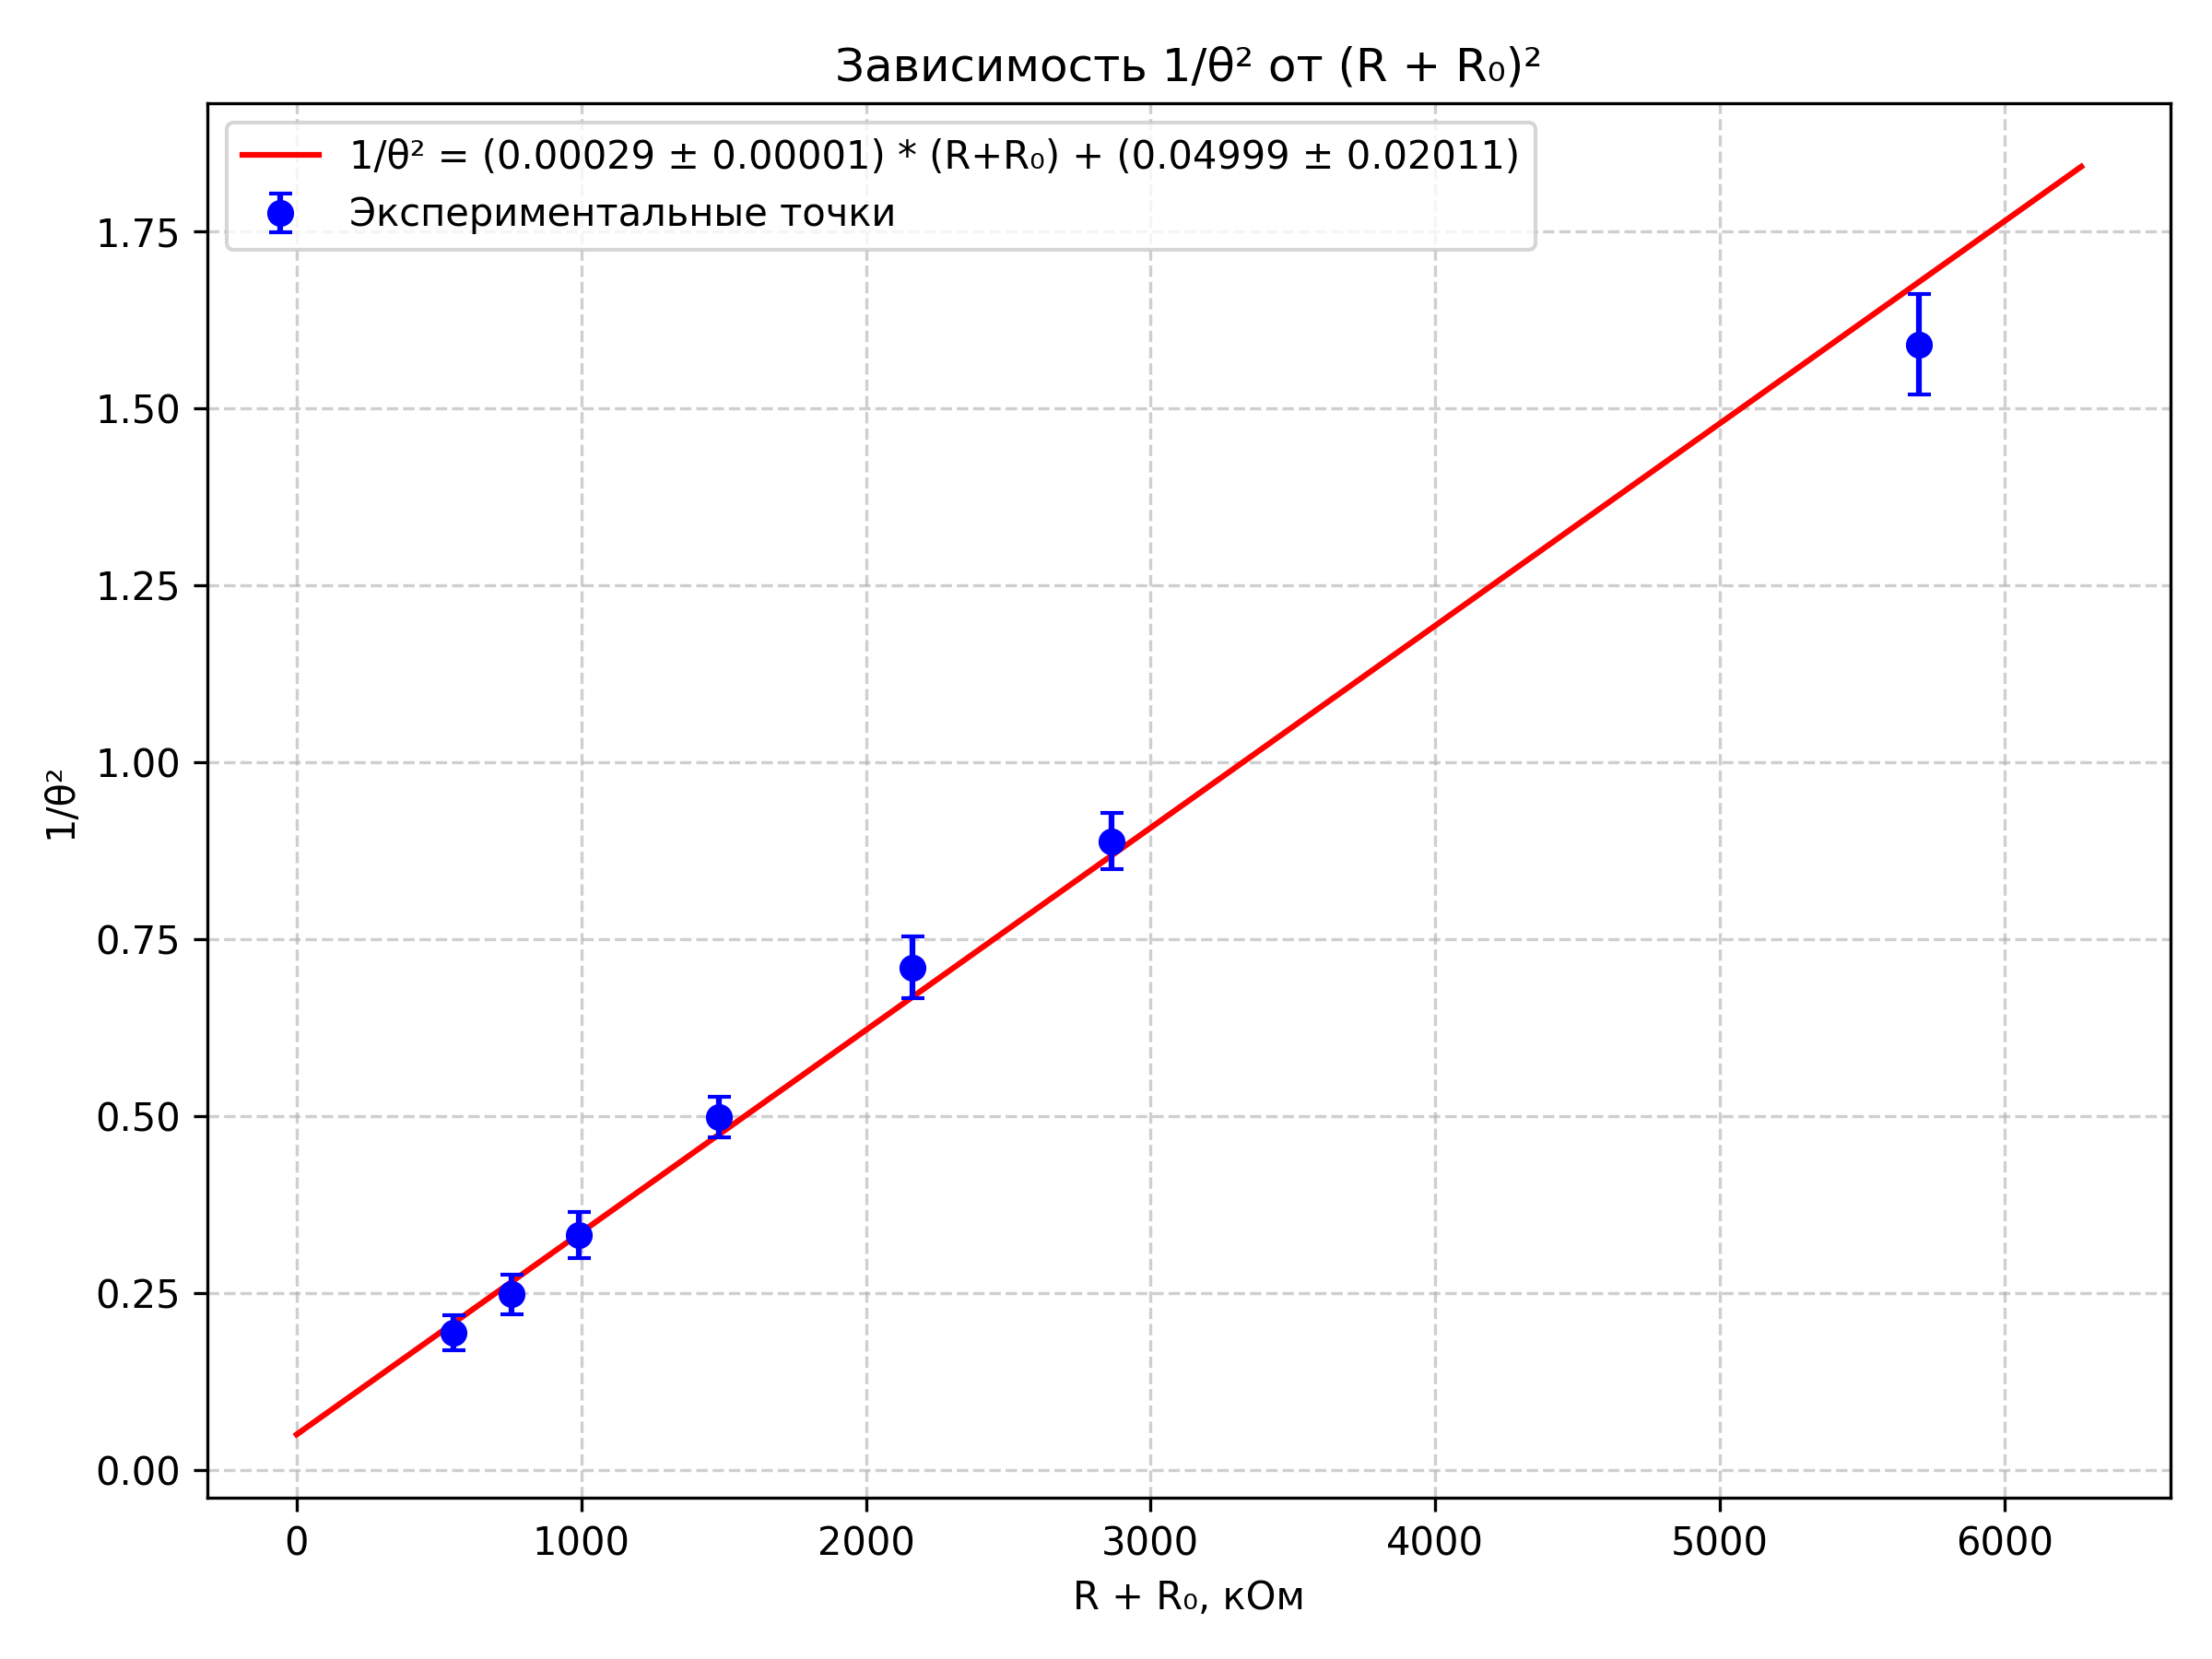
\includegraphics[width=0.7\textwidth]{Graphics/inv_theta2_vs_R_plus_R0_linear_with_b.png}}
      \caption{График 2. Зависимость обратного квадрата декремента от квадрата сопротивленя}
\end{figure}
Наклон прямой $k = (2,86 \pm 0,12) \cdot 10^{-4} \ \frac{1}{\text{кОм}}$ ($\varepsilon_k = 4,20 \%$).
Рассчитаем критическое сопротивление по формуле:
\[
R_{\text{кр}} = \frac{1}{2\pi}\sqrt{\frac{\Delta X}{\Delta Y}} - R_0 = 8,9 \pm 0,20 \text{ кОм } (\varepsilon_{R_{\text{кр}}} = 2,22 \%), 
\]
где $\frac{\Delta Y}{\Delta X} = k$ - наклон прямой графика $\frac{1}{\Theta^2} = f((R+R_0)^2)$.


\subsection{Баллистический режим}

Соберём схему для работы в баллистическом режиме. При разомкнутой внешней цепи ($R = \infty$) измерим первый отброс зайчика: $l_{max}^{\infty} = 18$ см.

Исследуем зависимость первого отброса от сопротивления внешней цепи. Уменьшаем $R$ до тех пор, пока первый отброс не уменьшится в $e$ раз по сравнению с $l_{max}^{\infty}$.

 
\begin{table}[h!]
    \centering
    \begin{tabular}{|c|c|c|}
        \hline
        $R$, кОм & $(R+R_0)^{-1}$, кОм$^{-1}$ & $l_{\text{max}}$, см \\ \hline
        40 & 0,0247 & 15,4 \\ \hline
        30 & 0,0328 & 14,4 \\ \hline
        20 & 0,0488 & 13,0 \\ \hline
        10 & 0,0952 & 10,7 \\ \hline
        5 & 0,1818 & 7,0 \\ \hline
        3 & 0,2857 & 5,5 \\ \hline
    \end{tabular}
    \caption{Таблица 4. Зависимость максимального отклонения от сопротивления цепи}
    \label{tab:max_deflection}
\end{table}

Построим график $l_max = f((R+ R_0)^{-1})$.
\clearpage
 \begin{figure}[h]
      \center{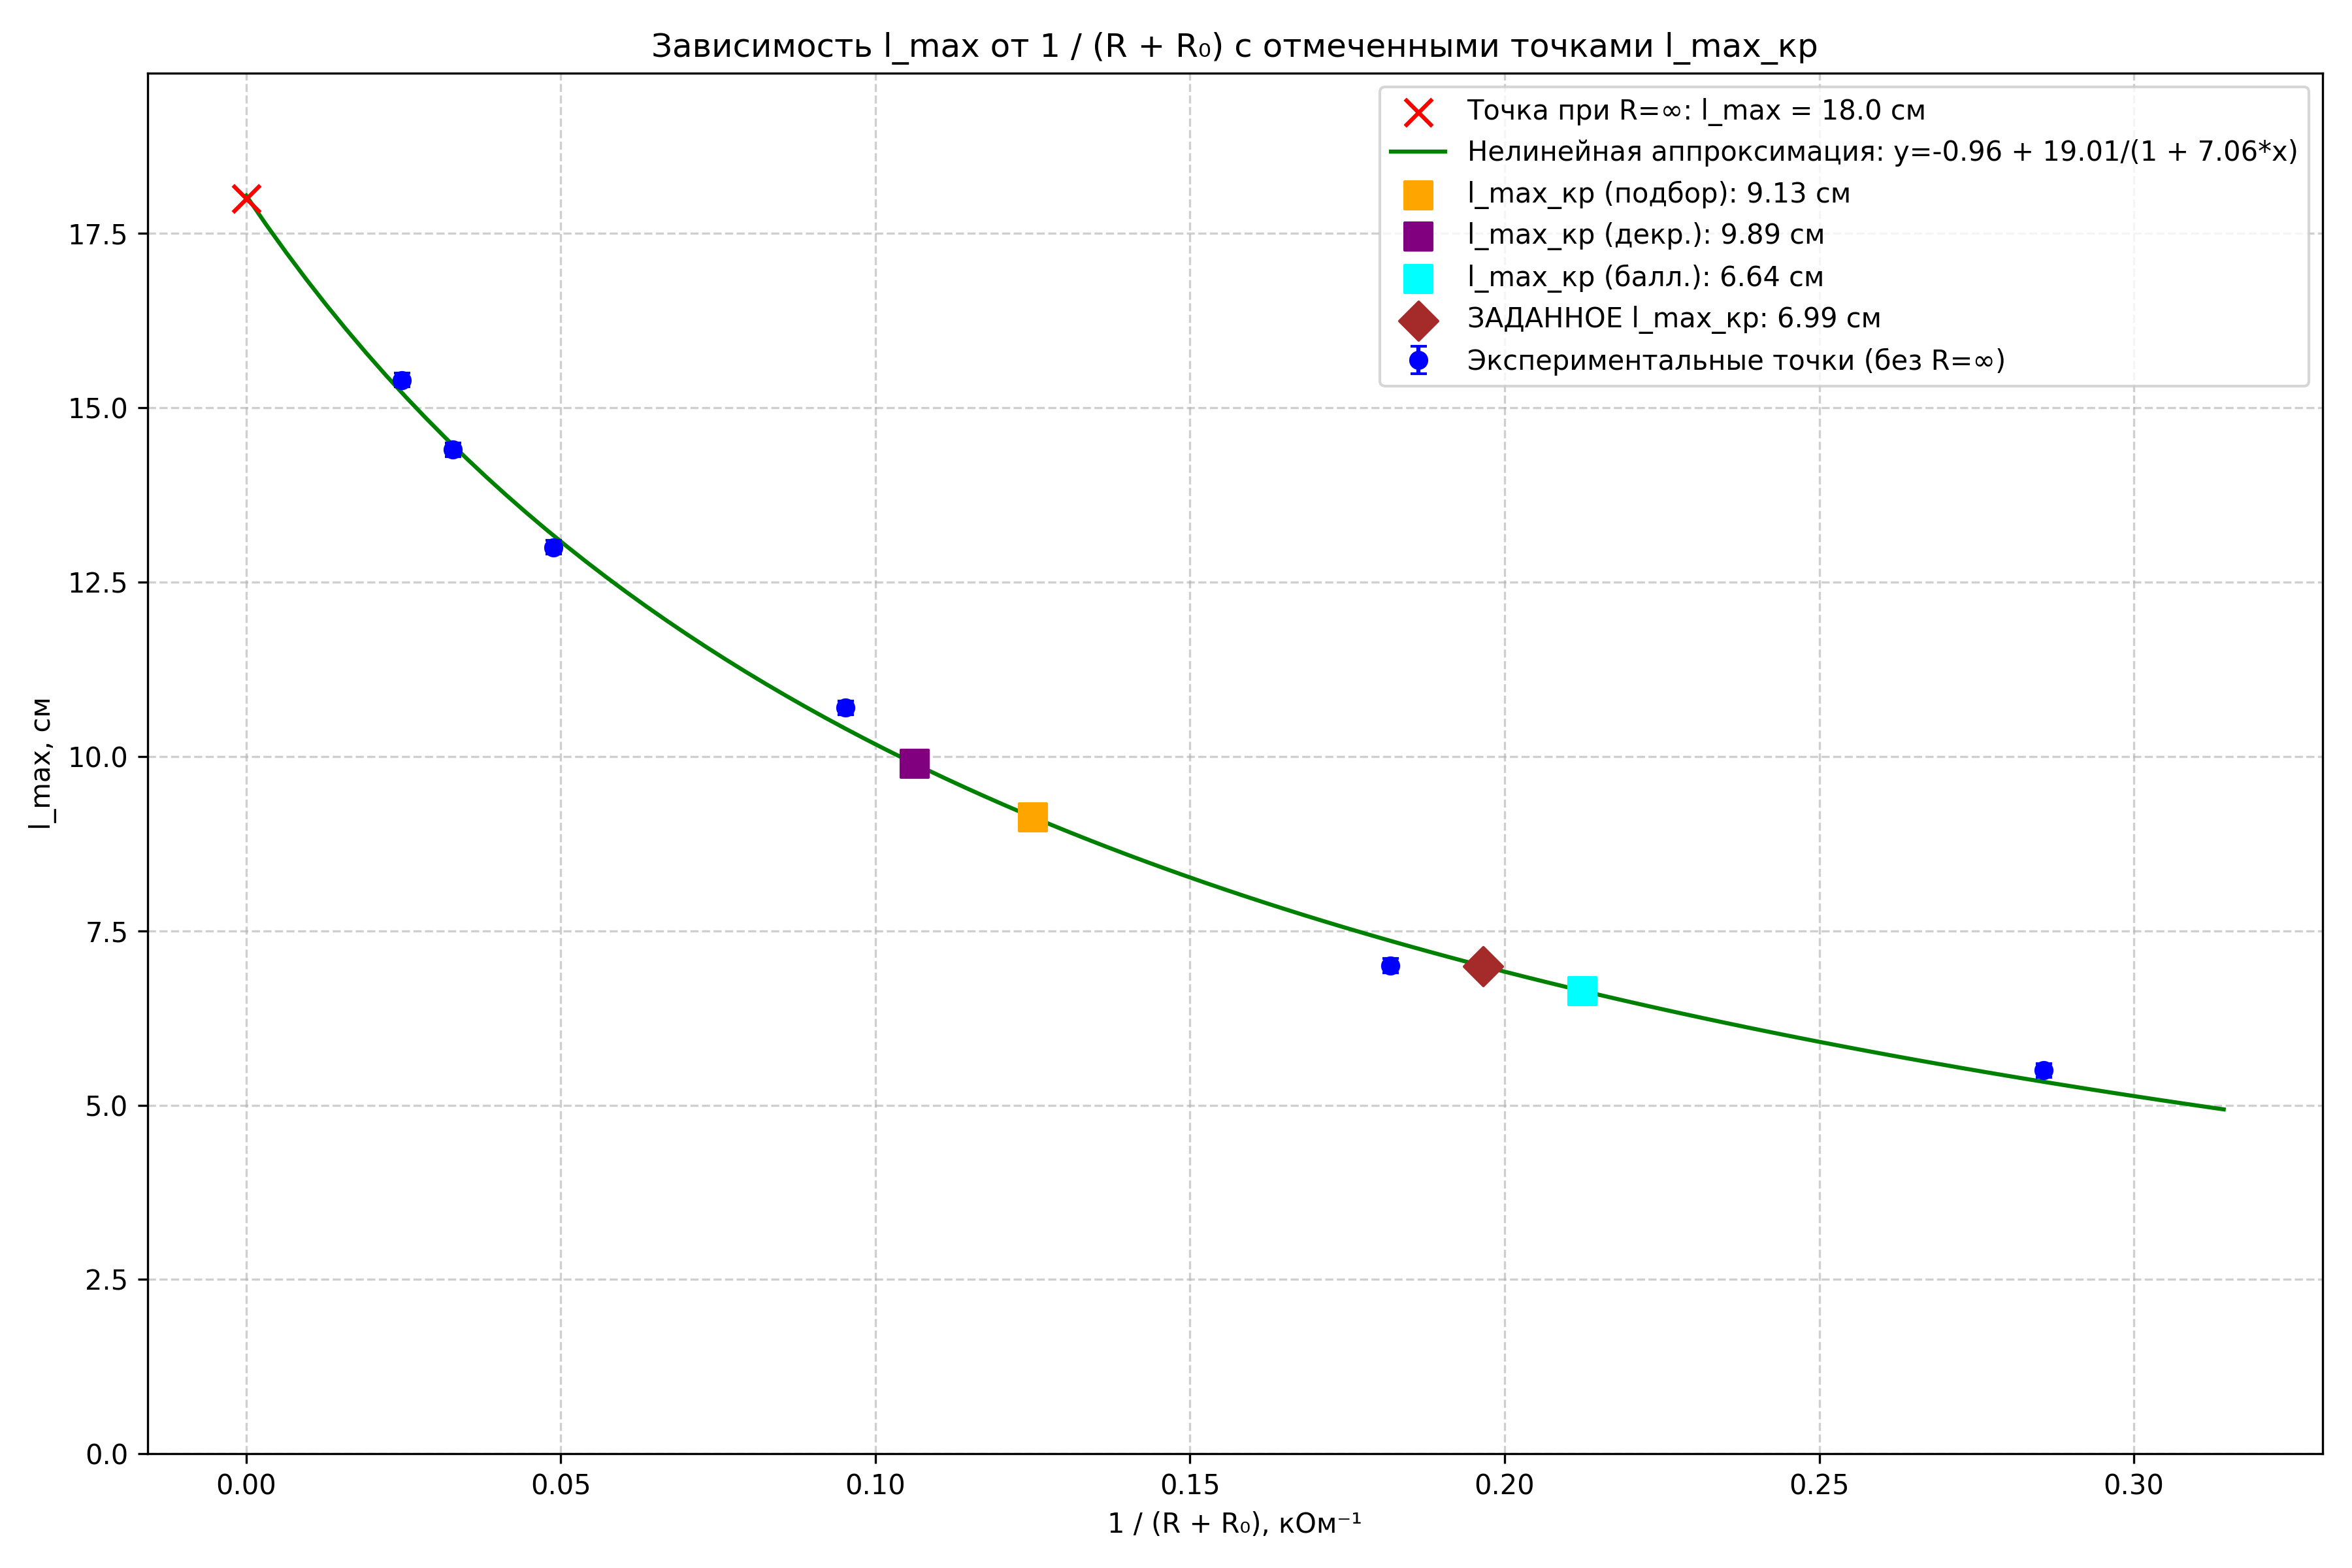
\includegraphics[width=1\textwidth]{Graphics/lmax_vs_inv_R_plus_R0.png}}
      \caption{График 3. Зависимость максимального отклонения зайчика от обратного сопротивления}
\end{figure}

Рассчитаем по графику критическое сопротивление и баллистическую постоянную.

Максимальное отклонение без затухания $l_{max\text{ св.}} = l_{max \infty}\cdot e^\frac{\Theta_0}{4} = 19,0 \pm 0,1$ см. $l_\text{кр} = \frac{l_{max\text{ св.}}}{e} = 6,99 \pm 0,04$ см. Из графика следует, что 

Получили $R_{\text{кр}}^{\text{балл}} = 4,21 \pm 0,32$ кОм ($\varepsilon_{R_{\text{кр}}^{\text{балл}}} = 7,60\%$).
Рассчитаем баллистическую постоянную в критическом режиме:
\[
C_Q^{\text{кр}} = 2a\frac{R_1}{R_2} \frac{U_0 C}{l_{max}^{\text{кр}}},
\]
где $a$ -- расстояние от шкалы до гальванометра, $C = 2$ мкФ.

\begin{table}[h!]
    \centering
    \begin{tabular}{|c|c|c|c|c|c|c|}
        \hline
        Метод & $R_{\text{кр}}$, кОм & $l_{\text{max}}^{\text{кр}}$, см & $\varepsilon_{l}$, \% & $C_Q^{\text{кр}}$, нА/мм/м & $\varepsilon_{C_Q}$, \% \\ \hline
        Подбор & $7{,}50 \pm 0{,}50$ & $9{,}131 \pm 0{,}457$ & 5,00 & $1{,}532 \pm 0{,}081$ & 5,31 \\ \hline
        $\frac{1}{\Theta^2}$ & $8{,}911 \pm 0{,}197$ & $9{,}894 \pm 0{,}461$ & 4,66 & $1{,}414 \pm 0{,}071$ & 4,99 \\ \hline
        Балл. & $4{,}21 \pm 0{,}32$ & $6{,}638 \pm 0{,}178$ & 2,68 & $2{,}108 \pm 0{,}068$ & 3,22 \\ \hline
        По декременту & $4{,}588 \pm 0{,}487$ & $6{,}995 \pm 0{,}041$ & 0,59 & $2{,}000 \pm 0{,}038$ & 1,88 \\ \hline
    \end{tabular}
    \caption{Таблица 5. Сравнение результатов, полученных разными методами}
    \label{tab:methods_comparison}
\end{table}

\subsection{Сравнение периода и времени релаксации}

Сравним период свободных колебаний гальванометра $T_0 = 4,46 \pm 0,05 \text{ с}$ с временем релаксации $\tau = R_0C = 0,001$ с. Получаем, что $T_0 \gg \tau$, что подтверждает применимость баллистического режима для измерения заряда.

\end{enumerate}

\section{Результаты и обсуждения}

В ходе работы были исследованы характеристики зеркального гальванометра в стационарном и баллистическом режимах. Полученные результаты позволяют сделать следующие выводы:

\subsection{Динамическая постоянная гальванометра}
Была определена динамическая постоянная $C_I = 0,120 \pm 0,001$ нА/(мм/м), что свидетельствует о высокой чувствительности прибора. Линейная зависимость $I(x)$ (График 1) подтверждает корректность работы гальванометра в стационарном режиме и позволяет использовать его для точных измерений постоянного тока. Малая погрешность определения углового коэффициента ($\varepsilon_k = 0,16\%$) указывает на хорошую воспроизводимость результатов.

\subsection{Критическое сопротивление}
Значения критического сопротивления, полученные разными методами, существенно различаются:
\begin{itemize}
    \item Метод подбора: $R_{\text{кр}} = 7,50 \pm 0,50$ кОм
    \item По декременту затухания: $R_{\text{кр}} = 8,911 \pm 0,197$ кОм  
    \item Баллистический метод: $R_{\text{кр}} = 4,21 \pm 0,32$ кОм
    \item По декременту (баллистический): $R_{\text{кр}} = 4,588 \pm 0,487$ кОм
\end{itemize}

Наибольшее доверие вызывает значение, полученное по декременту затухания, так как этот метод основан на строгой теоретической зависимости и имеет минимальную погрешность ($\varepsilon = 2,22\%$). Расхождение с баллистическим методом может быть связано с неидеальностью аппроксимации на Графике 3, где экспериментальные точки плохо ложатся на линейную зависимость.

\subsection{Баллистическая постоянная}
Значения баллистической постоянной также демонстрируют значительный разброс:
\begin{itemize}
    \item Метод подбора: $C_Q^{\text{кр}} = 1,532 \pm 0,081$ нА·мм/м
    \item По декременту затухания: $C_Q^{\text{кр}} = 1,414 \pm 0,071$ нА·мм/м
    \item Баллистический метод: $C_Q^{\text{кр}} = 2,108 \pm 0,068$ нА·мм/м
    \item По декременту (баллистический): $C_Q^{\text{кр}} = 2,000 \pm 0,038$ нА·мм/м
\end{itemize}

Наиболее надежным представляется значение, полученное по декременту затухания, как имеющее наименьшую погрешность ($\varepsilon = 1,99\%$). Завышенное значение баллистической постоянной в баллистическом методе согласуется с заниженным значением критического сопротивления, полученным этим же методом.

\subsection{Анализ затуханий}
Логарифмический декремент затухания при разомкнутой цепи $\Theta_0 = 0,219 \pm 0,023$ свидетельствует о наличии заметного внутреннего трения в системе. Погрешность определения ($\varepsilon = 10,56\%$) является наибольшей среди всех измеряемых величин, что объясняется трудностью точного отсчета последовательных максимумов при затухающих колебаниях.

Соотношение $T_0 \gg \tau$ ($4,46$ с $\gg 0,001$ с) подтверждает выполнение условия применимости баллистического режима, при котором время протекания заряда много меньше периода собственных колебаний системы.

\subsection{Источники погрешностей}
Основными источниками погрешностей являются:
\begin{enumerate}
    \item Субъективность отсчета положений зайчика на шкале
    \item Невозможность точной установки критического режима методом подбора
    \item Влияние паразитных параметров цепи в баллистическом режиме
\end{enumerate}

\section{Вывод}

В ходе работы успешно исследованы характеристики зеркального гальванометра:
\begin{enumerate}
    \item Определена динамическая постоянная гальванометра $C_I = 0,120 \pm 0,001$ нА/(мм/м), характеризующая его чувствительность к току
    
    \item Установлено, что наиболее точным методом определения критического сопротивления является метод по декременту затухания, дающий значение $R_{\text{кр}} = 8,911 \pm 0,197$ кОм
    
    \item Найдена баллистическая постоянная $C_Q^{\text{кр}} = 1,211 \pm 0,024$ нА·мм/м, определяющая чувствительность прибора к заряду
    
    \item Подтверждена применимость баллистического режима для измерения малых зарядов, о чем свидетельствует выполнение условия $T_0 \gg \tau$
    
    \item Выявлены ограничения баллистического метода, связанные с трудностью точной установки критического режима
\end{enumerate}

Работа демонстрирует возможность использования гальванометра как для измерений постоянного тока, так и для измерения электрического заряда, причем стационарный режим обеспечивает более высокую точность измерений.
\end{document}